\begin{problem}{Margföldun}{Inn}{Út}{~}{~}
	
	\begin{wrapfigure}{r}{0.35\textwidth}
		\vspace{-25pt}
		\begin{center}
			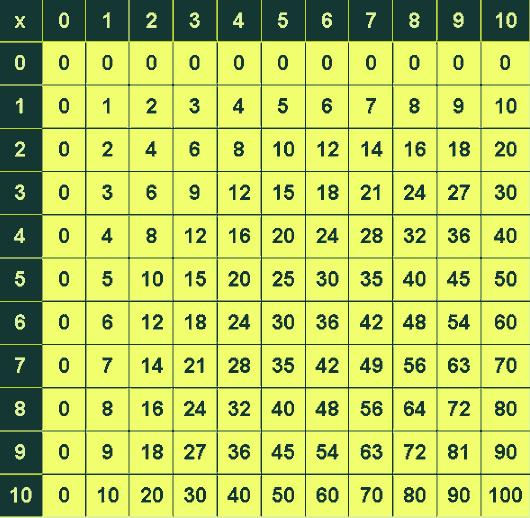
\includegraphics[scale=0.4]{../Margfoldun/table.jpg}
		\end{center}
		\vspace{-30pt}
	\end{wrapfigure}

	Jón litli er búinn að læra samlagningu og frádrátt í skólanum. Núna er hann að læra um margföldun, en hann er ekki enn búinn að ná fullkomnum tökum á henni (enda er margföldun margfalt erfiðari en samlagning). Hann er búinn að vera að æfa sig með því að taka tvær litlar tölur af handahófi og reyna svo að margfalda þær saman. Þegar hann er búinn að skrifa svarið niður, þá sannreynir hann það með því að nota vasareikninn sinn. En núna er hann í vandræðum, hann finnur ekki vasareikninn! Hvernig á hann þá að vita hvort svarið sé rétt eða ekki?

	Jón litli kemur til þín og biður þig um að skrifa forrit sem sannreynir svörin fyrir sig.

	\Input

		Á fyrstu línu er heiltalan $1 \leq T \leq 100$, sem táknar fjölda prófunartilvika sem fylgja. Hvert prófunartilvik samanstendur af einni línu með þremur heiltölum $0 \leq a,b < 100$ og $0 \leq c < 10000$, þar sem $a$ og $b$ eru tölurnar sem Jón er að margfalda saman, og $c$ er svarið sem Jón fékk. Heiltölurnar þrjár eru aðskildar með bili.

	\Output

		Fyrir hvert prófunartilvik á að skrifa út eina línu sem inniheldur "`\texttt{True}"' ef svarið sem Jón fékk er rétt, en "`\texttt{False}"' annars.

	\Examples

		\begin{example}
			\exmp{
5
8 3 24
6 7 43
0 8 1
17 13 221
1 1 1
			}{
True
False
False
True
True
}%
		\end{example}

\end{problem}